
\chapter{Prototype System}
%\index{TODO CHANGE: XYZ}
% NOTES / TODOs:
%
% Architecture scheme, implementation
% callback functions, hot plugin
% js-select selectors
% List of condition operators
% Why JS, why wasnt it used before? is it used now?
% Terminierungsproblem (compiler bau), loesungsansaetze

% Required use cases since their application was promised before in the thesis:
% smart filtering
% aggregation of information in whatever location user wants
% 

% as seen by user,
% as seen by developer

The prototype system is the realisation of a reactive Web system.
It was developped during the research for this thesis and acts as a platform for feasibility studies of certain use cases.

% FIXME remove
% \begin{table}[ht]
%   \centering
% 	\begin{tabular}{ l c r }
% 	  1 & 2 & 3 \\
% 	  4 & 5 & 6 \\
% 	  7 & 8 & 9 \\
% 	\end{tabular}
%   \caption{This table shows some data}
%   \label{tab:myfirsttable}
% \end{table}

% \section{Architecture}
Prototype consists of a queue in which all incoming events are pushed, and an engine that picks the events from the end of the queue whenever it is idle.
Since Prototype's core functionalty is the communication with resources in the Web, the architecture bases on HTTP protocol in several parts.
For example the events are meant to be retrieved completely via HTTP, the user interface is a Webpage which posts requests to the system and most actions are also meant to be HTTP requests, or at least using them to gather information.

% \begin{figure}[!ht]
% 	\centering
%   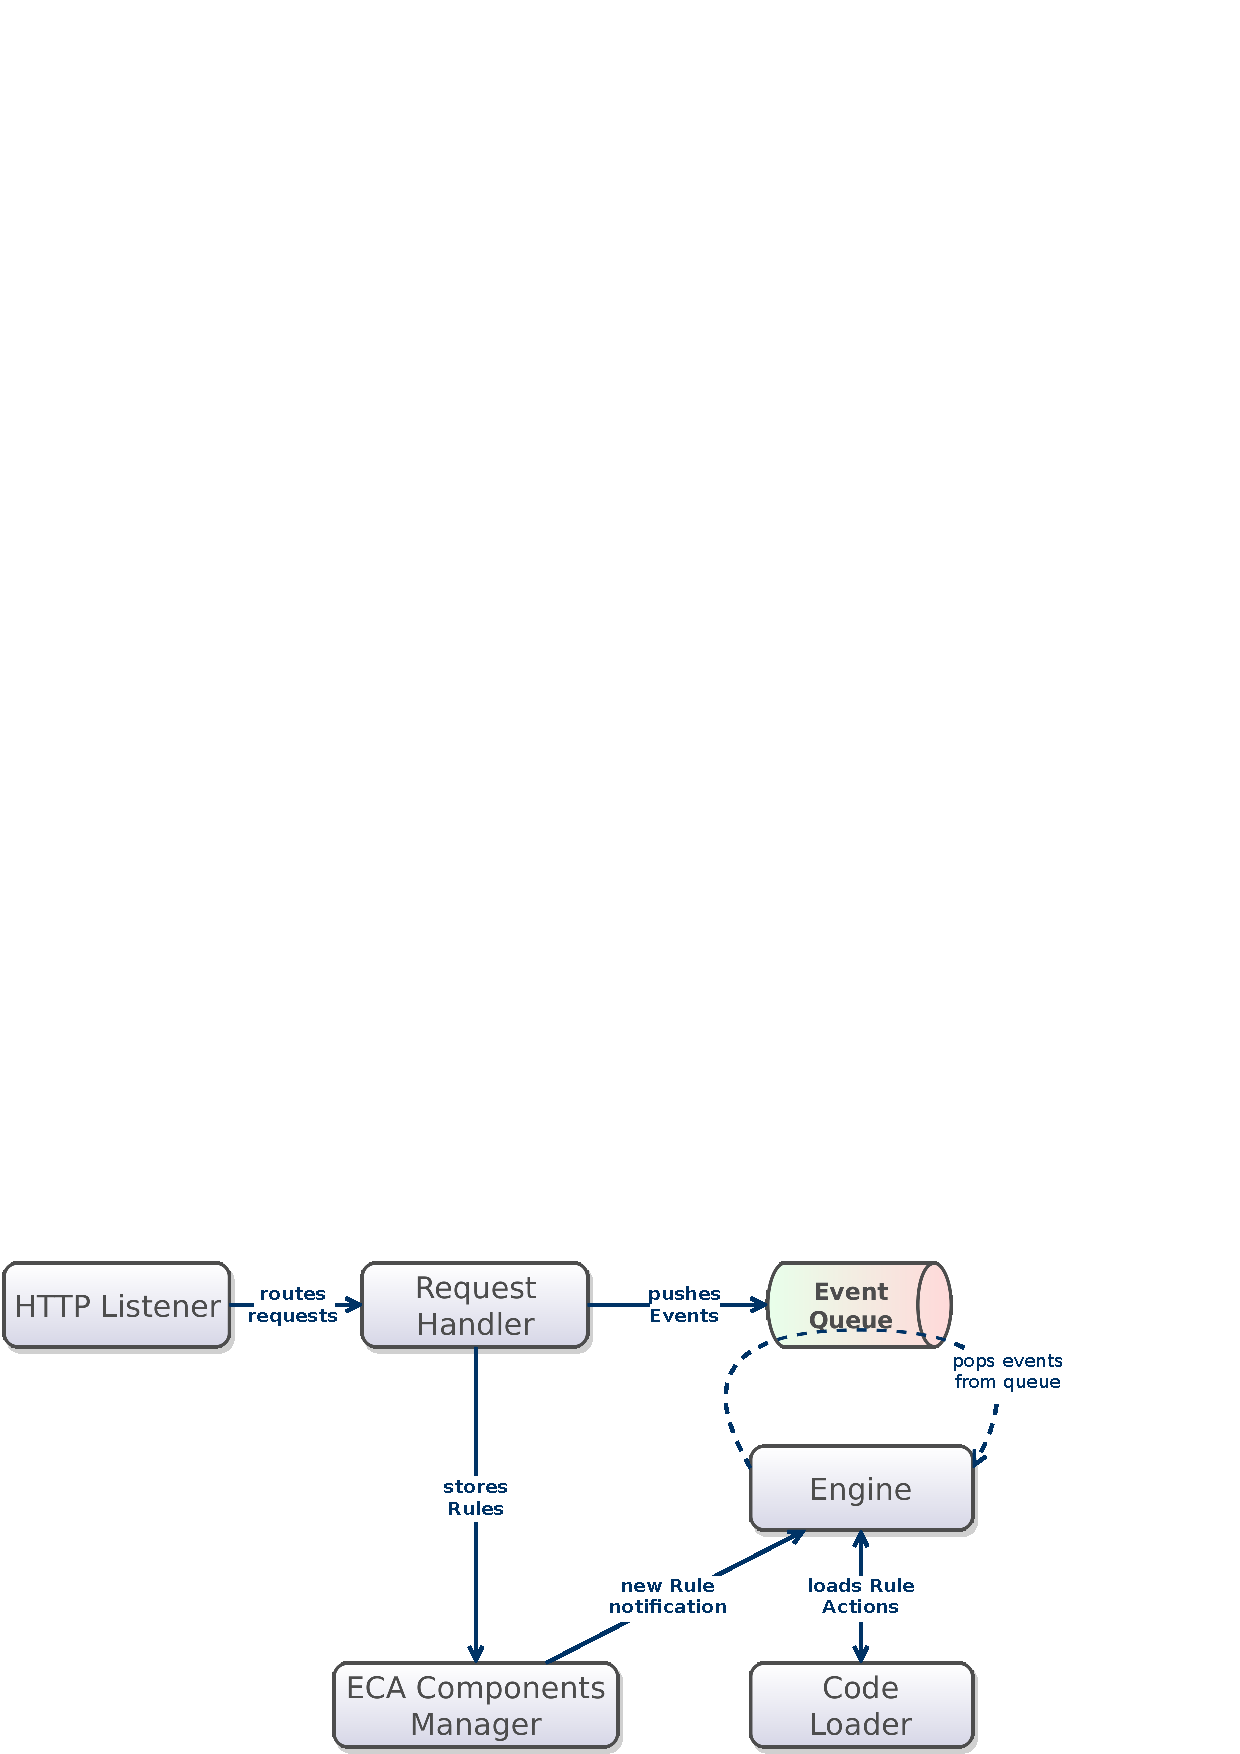
\includegraphics[width=0.8\textwidth]{figures/Architecture_woET}
% 	\caption{Prototype Architecture}
% 	\label{fig:Architecture_woEP}
% \end{figure}

Renew figure: (Rule Engine? Reactor?)
\begin{figure}[!ht]
	\centering
  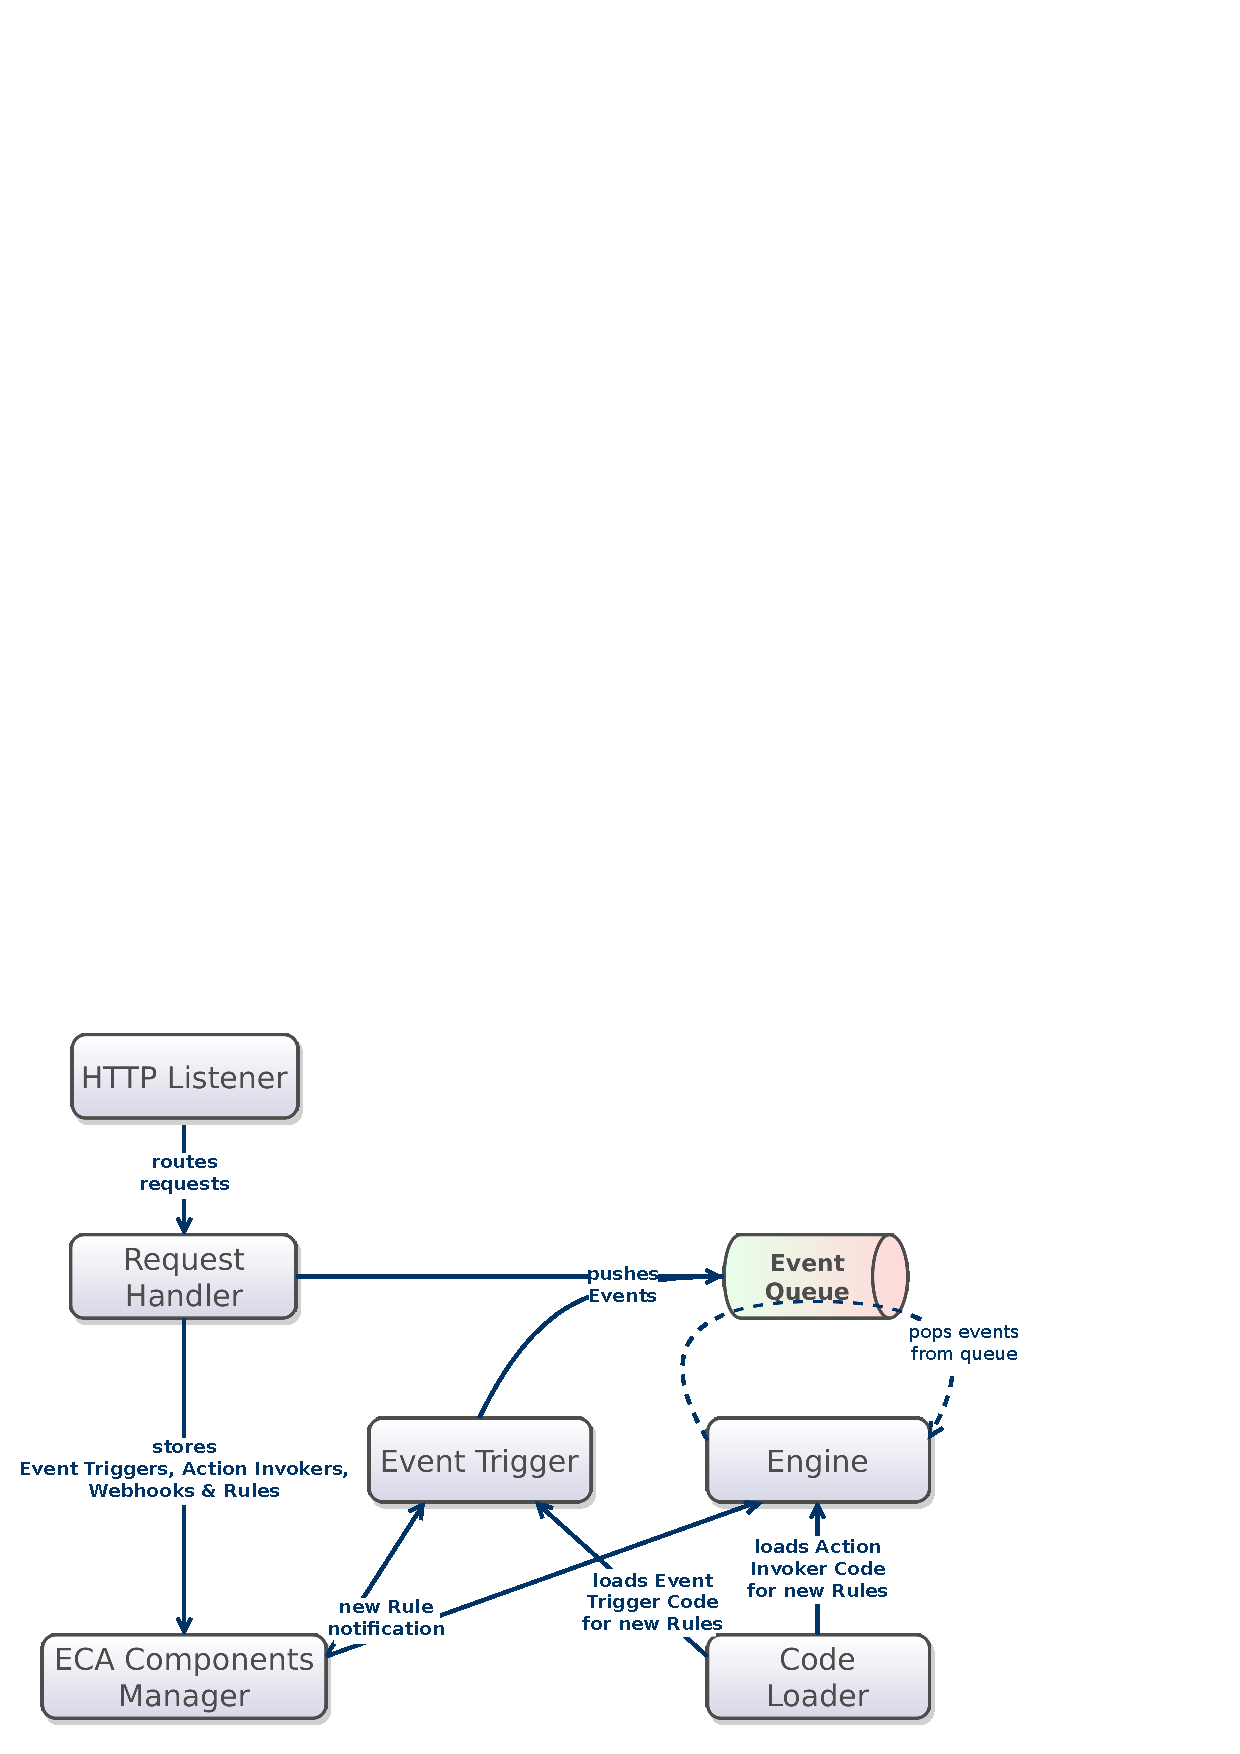
\includegraphics[width=0.9\textwidth]{figures/Architecture_wET}
	\caption{Prototype Process diagram}
	\label{fig:Architecture_wET}
\end{figure}


\section{Event Trigger}

Event Gathering is the E in ECA and without one of these letters such a system would not run.
It is of utmost importance to find as much as possible ways to get data into a system.



\subsection{Polling}

\subsection{Webhooks}







\section{Action Dispatcher}

% Not only from events
% import.io

\section{ECA Rules in the Engine}
% TODO Conditions

% vague Rule language limited through user acounts to not harm the system
% Describe possible attacks
% is descriptive, adaptive, flexible

% Explain rules, transferrability to language?

% dynamic code modules to shield system from user modules

%explain modules and their properties / user associations




% Apply variable number of function arguments to function

% \section{Grab data from anywhere}

% TODO figure: Wer hat welche rollen?
% TODO figure: Event fluss in verschiedenen UCs
% TODO figure: event anomalien (3-4 knoten)
% TODO figure: Unterschied Push / Pull -> unter introduction bei Webhooks?

% Callbacks / Webhooks semantical similarities but at different layers





\section{Concrete Use Cases?}
% holiday tips (Weather better somewhere else) if calendar empty

% Kalender eintrag fahrt in den süden, informaieren über offene pässe

% Regionalisierte news (news ratings)



During our research we found a troublesome server room that shows how the \textrm{Web of Things} can be exposed through our model.
This server room suffered from a defective cooling system which lead to a drastical increase of temperature in certain circumstances.
As a consequence certain server automatically shut themselves down as safety measurements.
Eventually, these shutdowns weren't detected immediately by the people that administered these servers, therefore unnecessary downtimes were the result.
As a very quick fix to inform certain administrators about the shutdown of their server, we started pinging these servers and pushed the results int



\section{Web Programming}


\subsection{Node.js}
% Why JS, why wasn't it used up to now? is it used now?

% TODO Take from preparation

% TODO figure: Callback; Result ensurance (ergebnissichherung) wird direkt mit funktion mitgeschickt

% Umgang mit der Zukunft
% Callback
\subsection{Callback Functions}

\subsection{Asynchronous Closures}
% JAva futures? objekte für resultate sammeln

% NOTES / TODOs:
%
% Variable bindings
% Closures (https://developer.mozilla.org/en-US/docs/Web/JavaScript/Guide/Closures)$
% Closures are functions that refer to independent (free) variables. 
% In other words, the function defined in the closure 'remembers' the environment in which it was created in.

% write about arallel as well?

Often, optimization approaches and programming language concepts require special attention to avoid common pitfalls.
When closures are used as asynchronous functions, developers need to be very careful not to end up with race conditions.


Looking at an example of sequential code execution in Figure~\ref{fig:Closures_Synchronous}, we see that function execution of \texttt{fA} is halted until function \texttt{fB} is finished.
If \texttt{fB} happens to be a latency-driven I/O operation the completion of \texttt{fA} could be deferred for a relatively long time.
While the application waits for the completion of the I/O operation, some remaining operations in \texttt{fA} could eventually already be executed without causing any race conditions.
\begin{figure}[!ht]
	\centering
  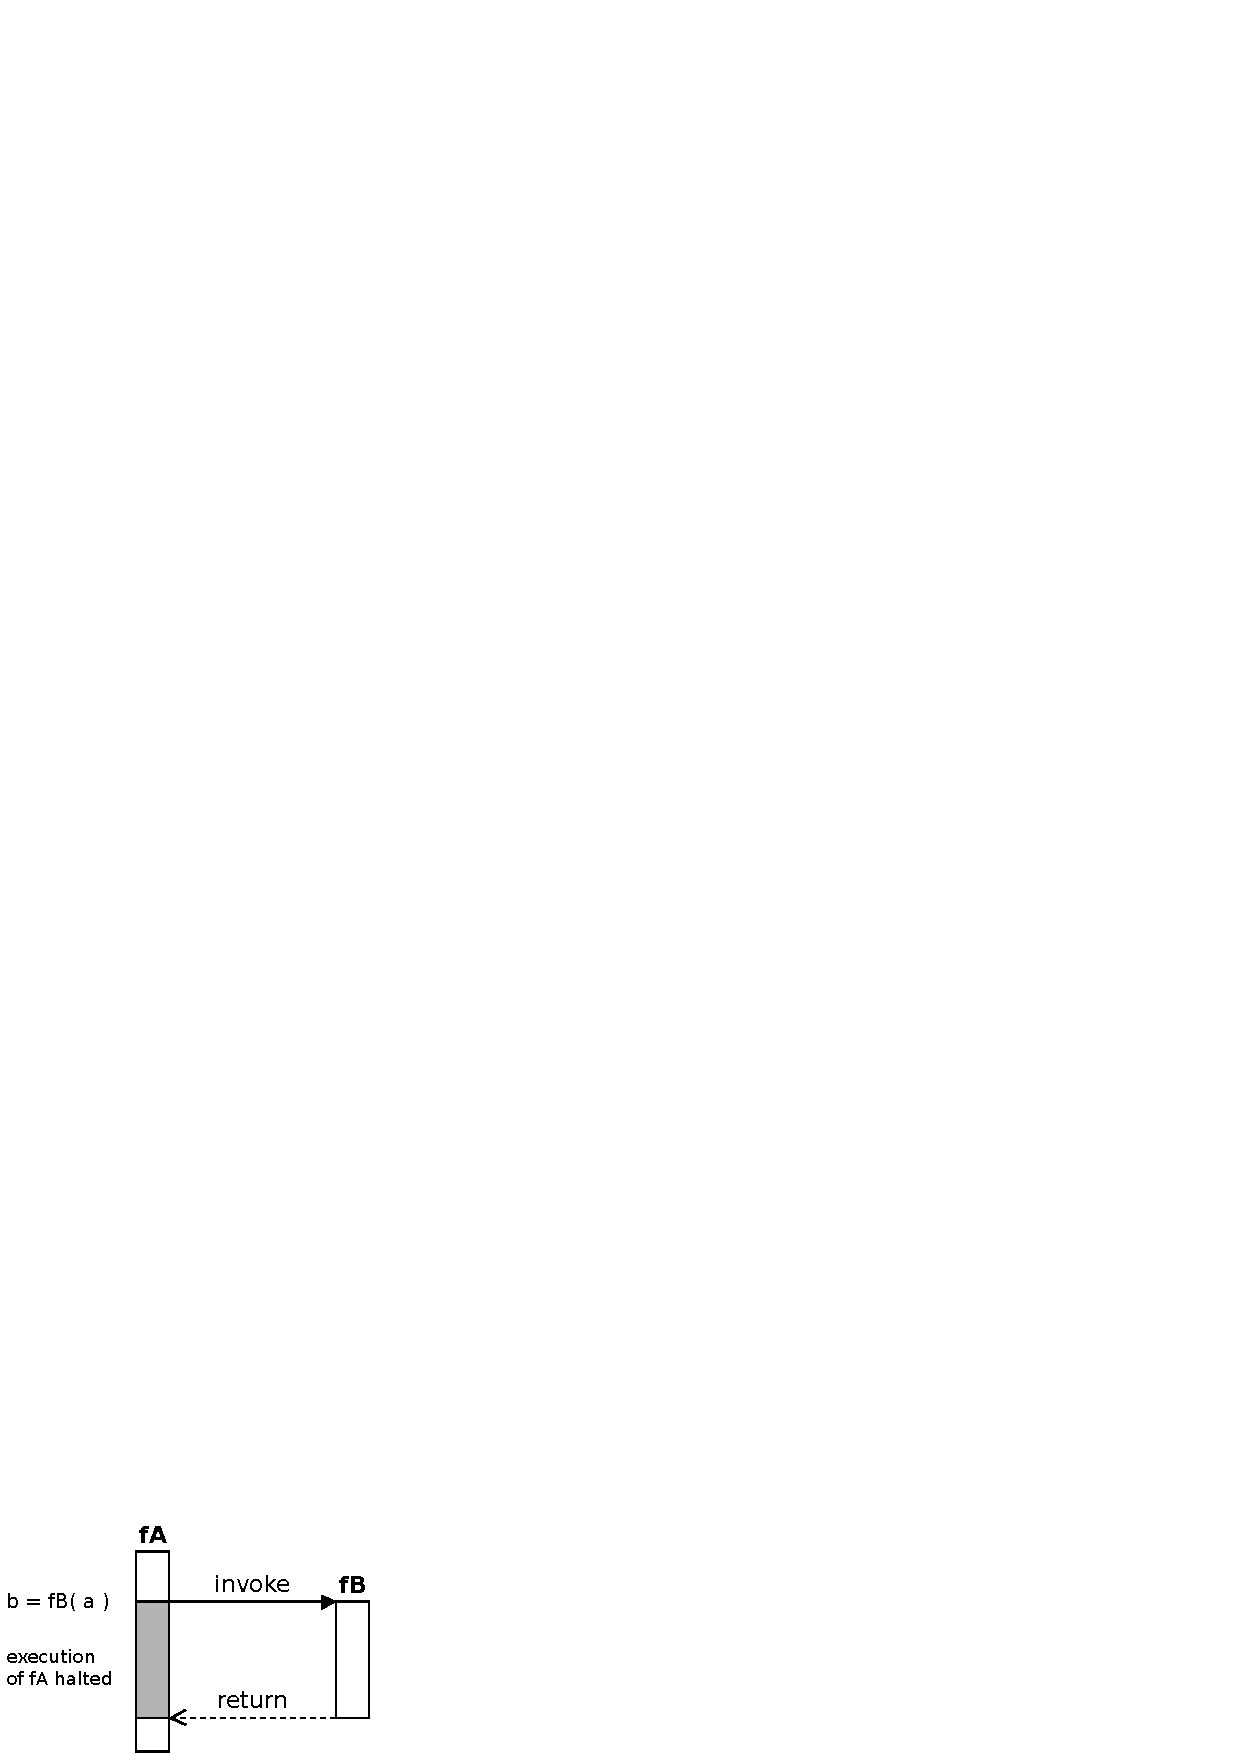
\includegraphics{figures/Closures_Synchronous}
	\caption{Synchronous Function Call}
	\label{fig:Closures_Synchronous}
\end{figure}


Asynchronous code execution, as shown in Figure~\ref{fig:Closures_Asynchronous}, allows non-blocking and thus scalable applications.
Non-blocking operations are a remedy for optimzed resource allocation and open up ways to overcome previously described unnecessary resource bindings.
Processing any kind of latency-driven I/O operation asynchronously ( e.g. filesystem access and socket communication ) exploits resources that would otherwise be bound while waiting for completion.
Such operations are processed and completed whenever required resources are available.
\begin{figure}[!ht]
	\centering
  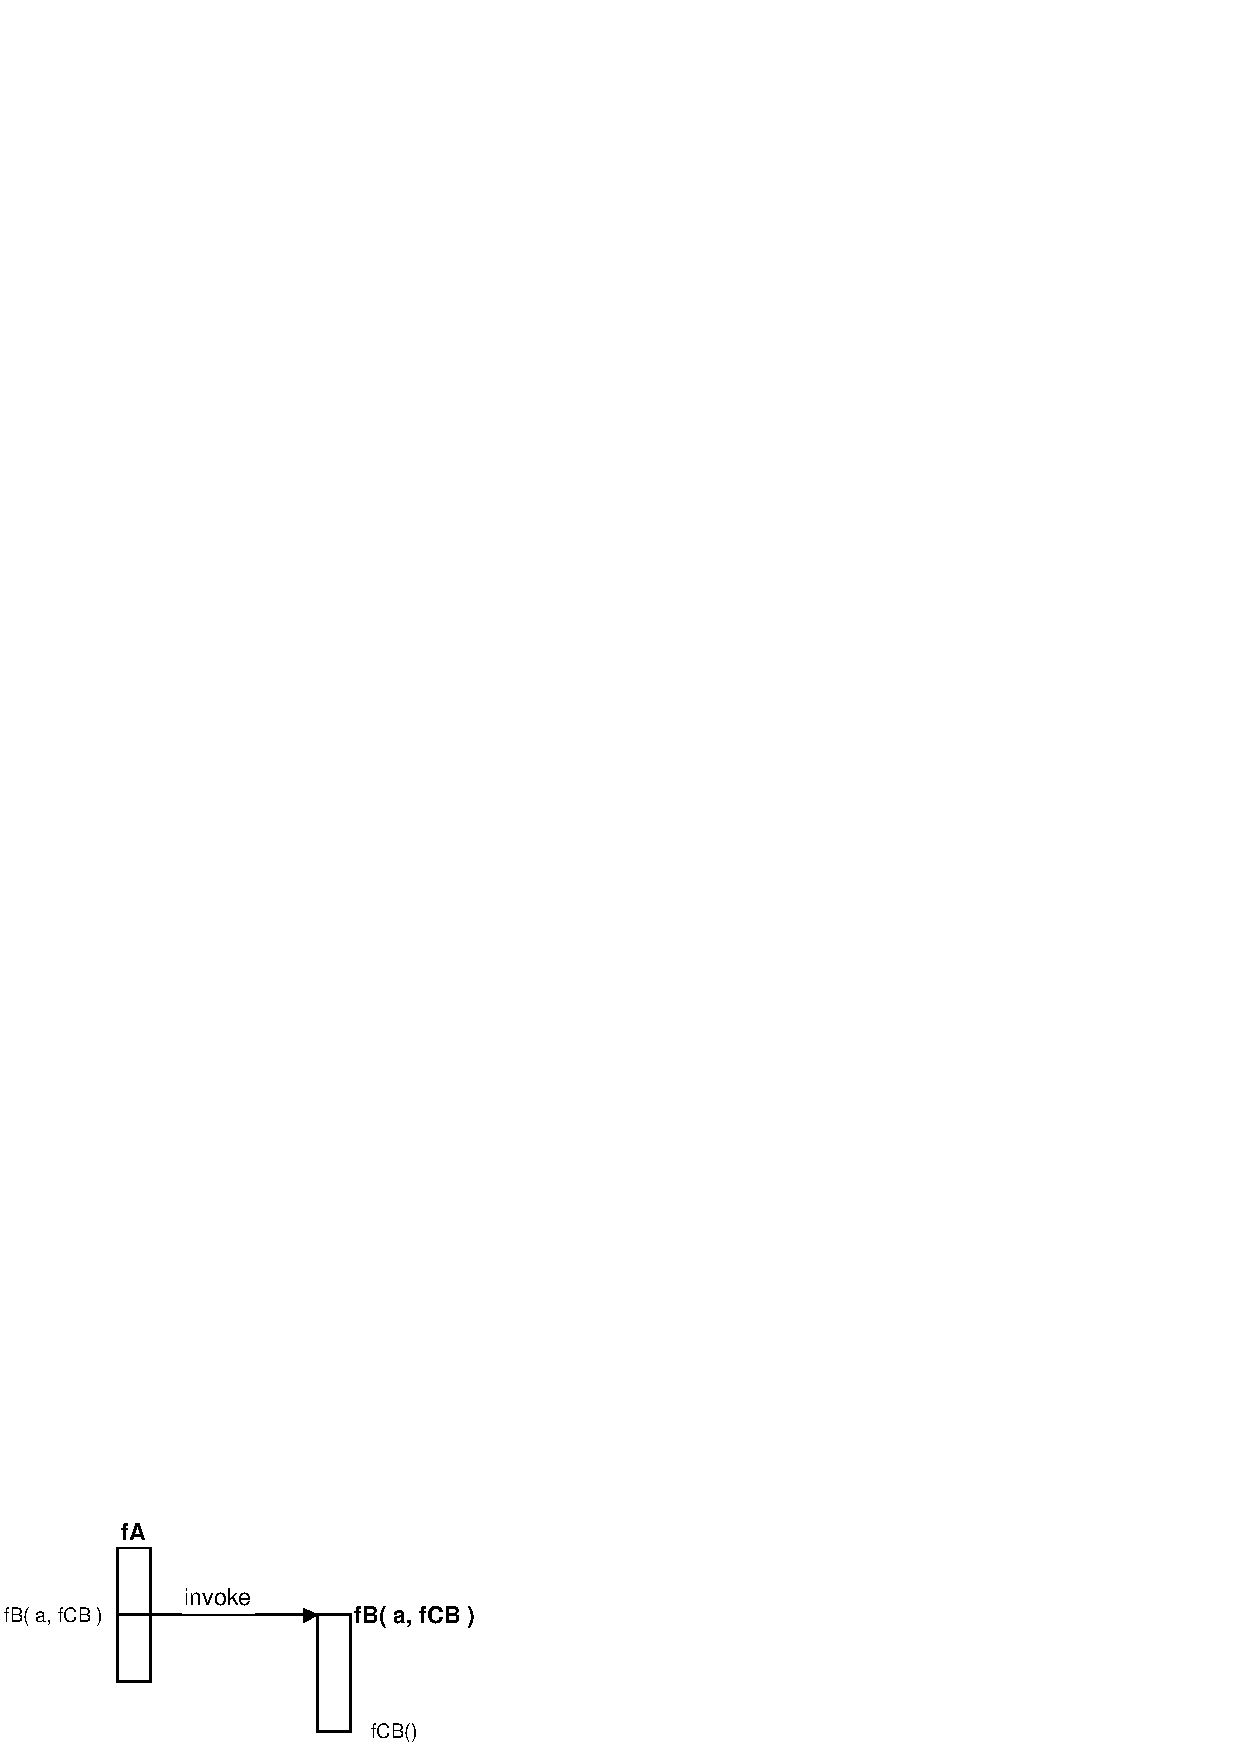
\includegraphics{figures/Closures_Asynchronous}
	\caption{Asynchronous Function Call}
	\label{fig:Closures_Asynchronous}
\end{figure}


Often other operations depend on the completion of asynchronous operations, hence their execution needs to be deferred.
This necessary code execution deferral is achieved through the use of callback functions, denoted \texttt{fCB} in Figure~\ref{fig:Closures_Asynchronous}.
Any code placed in a callback function, which is assigned to an asynchronous operation, is only executed after the respective asynchronous operation completed.
This allows stacking of functions and operations upon each other which automatically results in a flexible and event-driven application.


Now we take closures into this asynchronous context, as defined in ECMAScript\cite{EcmaScript}, which is the base for widely-spread script languages like JavaScript, JScript and ActionScript.
Closures in ECMAScript\cite{EcmaScript} are defined such as they have access to the context of the function they were created in.
This is shown in Figure~\ref{fig:Closures_Closure-1} where \texttt{c} from \texttt{fA}'s context is accessible from within \texttt{fB}, assuming that \texttt{fB} was created in \texttt{fA} and not only invoked from there.
Using asynchronous closures it becomes evident, that the context in the invoking function can change while the closure is still computing and eventually referencing the outer context, thus causing race conditions.
This will be most obvious in a loop that immediately invokes \texttt{fB} several times, as shown in Figure~\ref{fig:Closures_Closure-2}.
In such a setup \texttt{c} will have different values in the same part of different invocations of \texttt{fB}.
\begin{figure}[!ht]
	\centering
  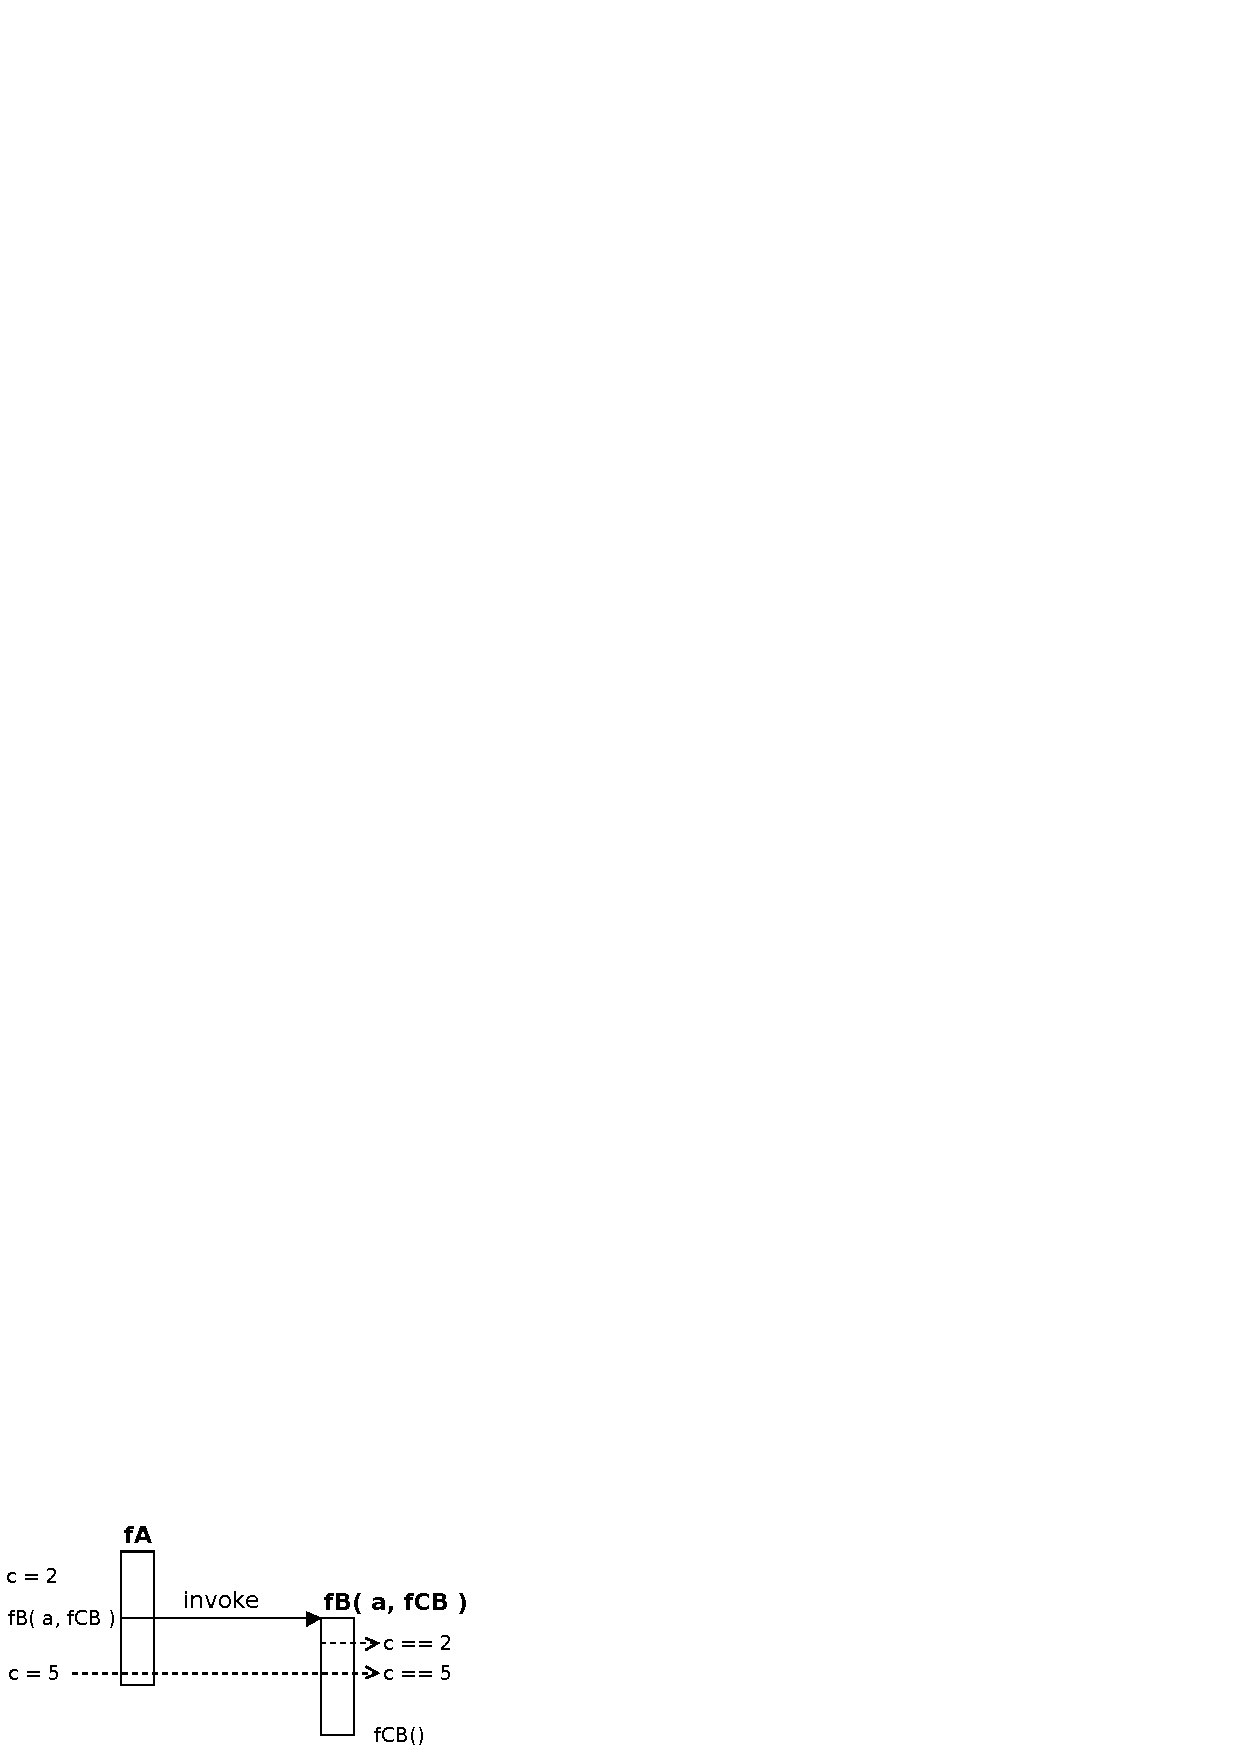
\includegraphics{figures/Closures_Closure-1}
	\caption{Closure Scope and referenced context}
	\label{fig:Closures_Closure-1}
\end{figure}
\begin{figure}[!ht]
	\centering
  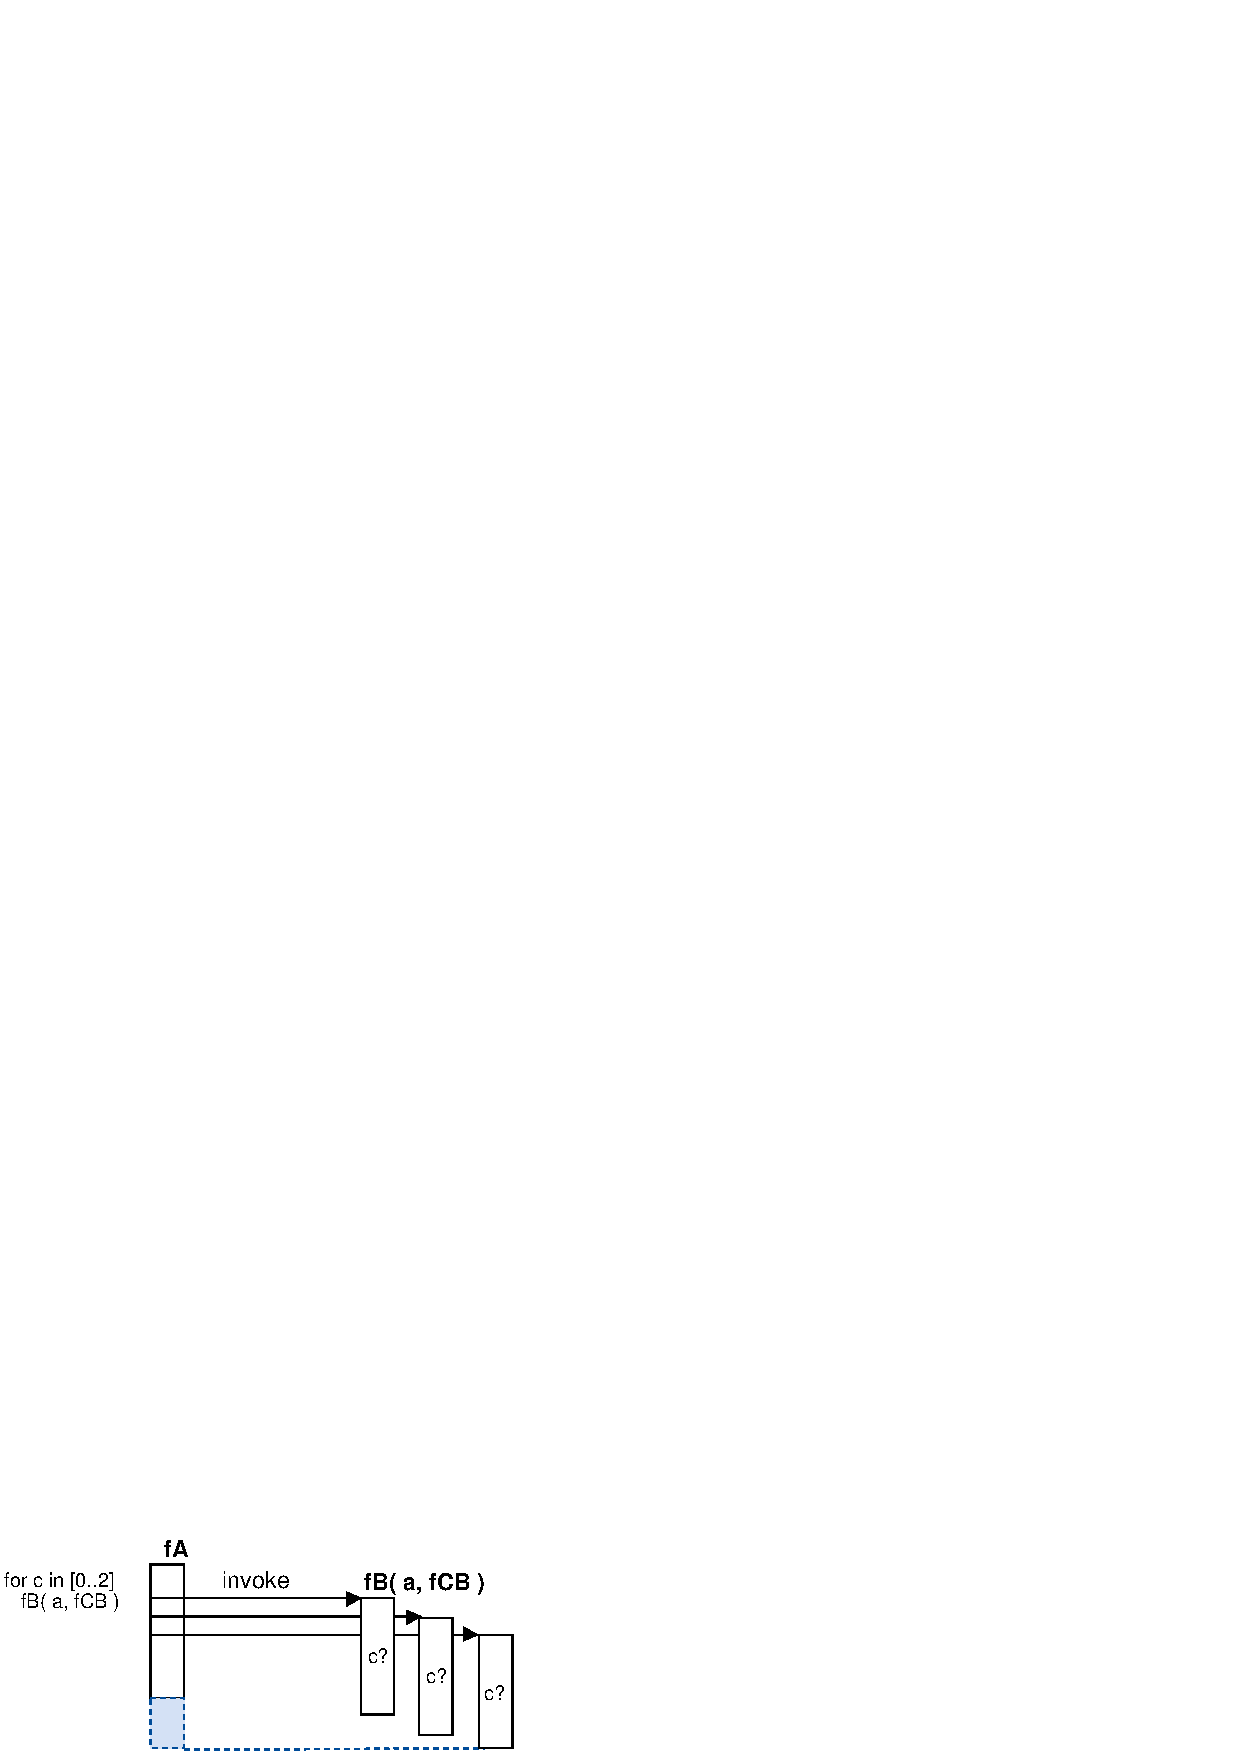
\includegraphics{figures/Closures_Closure-2}
	\caption{Closure context changes in a loop}
	\label{fig:Closures_Closure-2}
\end{figure}


Those event-driven context overwrites can be taken care of by shielding the closure from context changes, as shown in Figure~\ref{fig:Closures_Closure-3}.
To shield the closure form context changes, closure \texttt{fB} needs to create another closure \texttt{fC} and return it to \texttt{fA}.
The argument passed to \texttt{fB} is the context ( \texttt{c} in Figure~\ref{fig:Closures_Closure-3} ) that might change but requires to be persistent for one invocation.
\texttt{fC} has now \texttt{c} as a fixed context, which can't be overwritten anymore.
Now the only thing left is \texttt{fC} needs to be invoked and it will retain the original context.
This implementation is necessary when the closure acts as a callback function for asynchronous operations, to preserve the original context in case it is required within the callback function.
\begin{figure}[!ht]
	\centering
  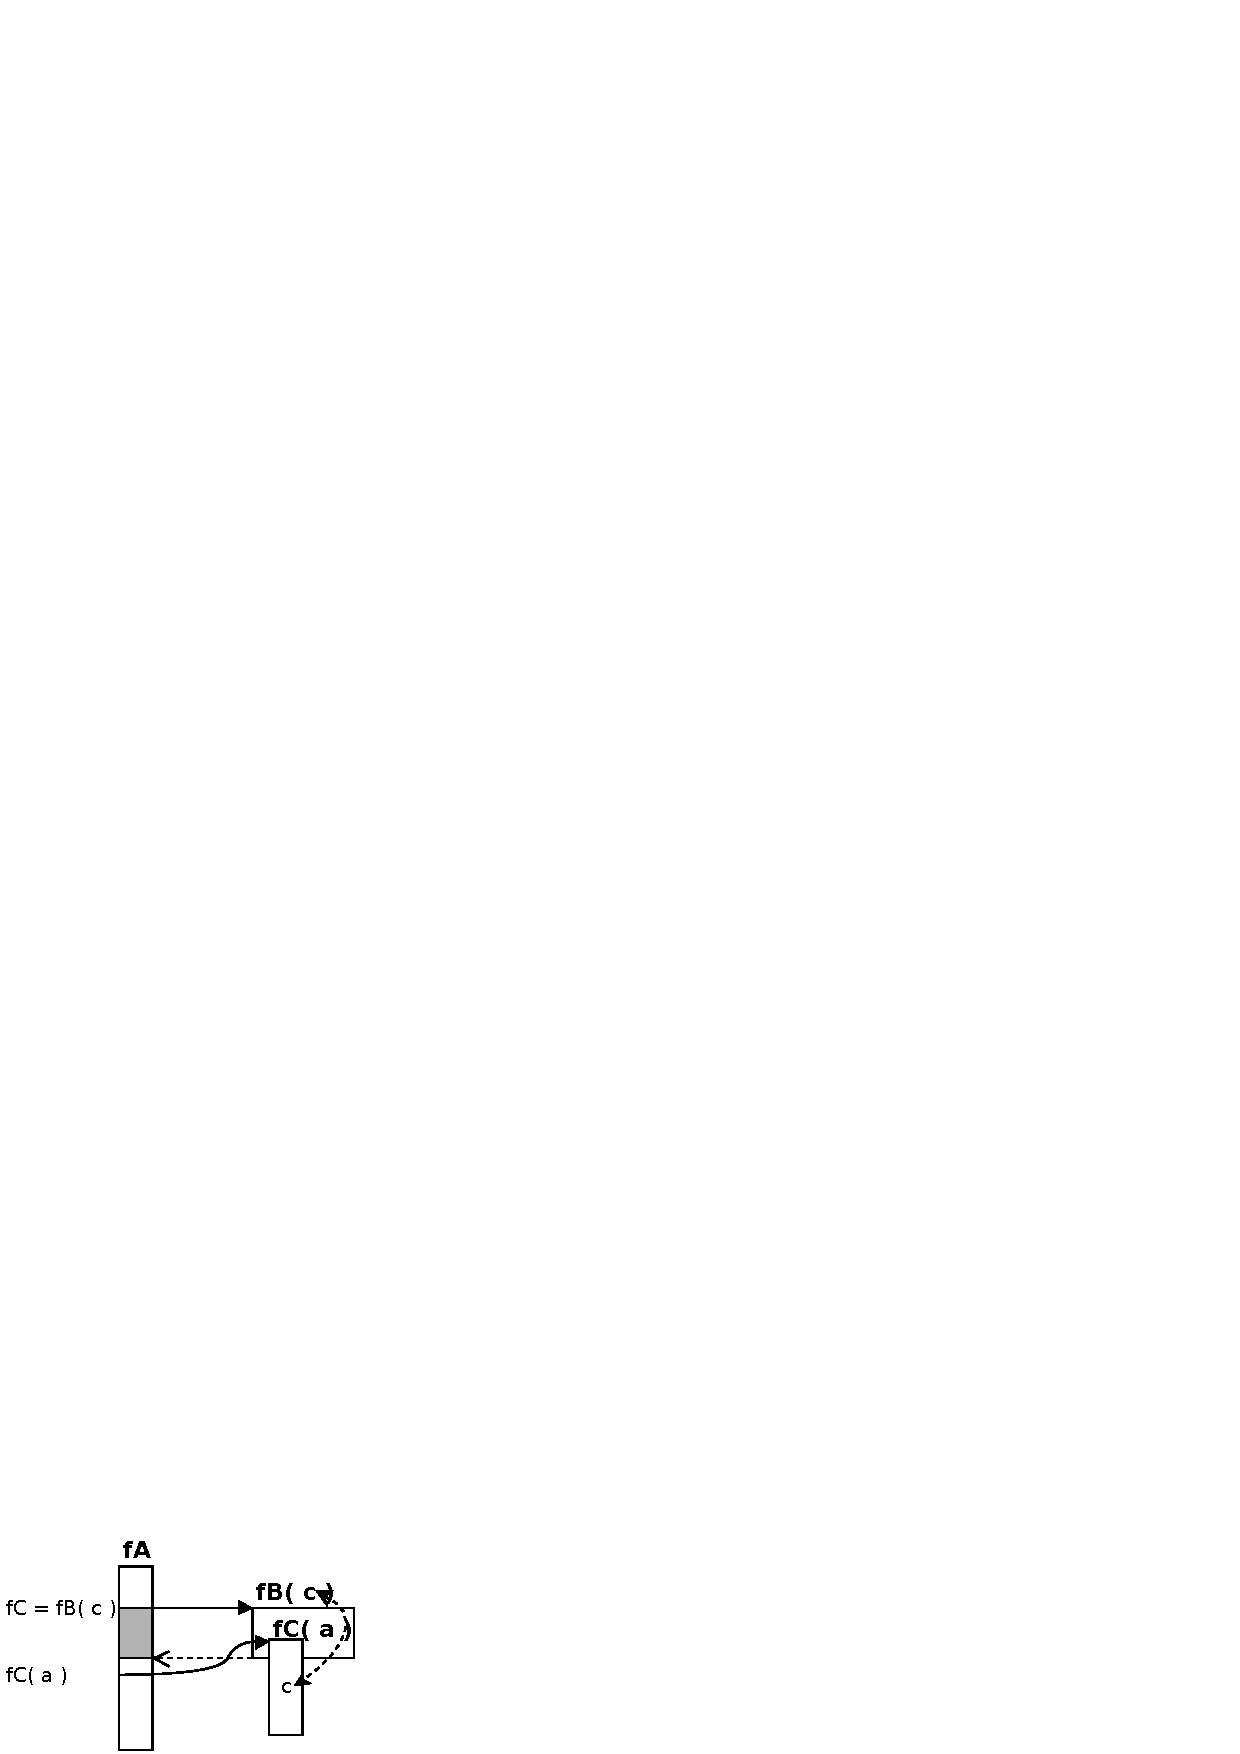
\includegraphics{figures/Closures_Closure-3}
	\caption{Closure context shielding}
	\label{fig:Closures_Closure-3}
\end{figure}

% TODO try async closures in other programming languages


\subsubsection{Benchmarking JavaScript vs. Java}
refer to listings
% TODO terminierungsproblem, testing, Web server, timeout, stacked callbacks.
%compilerbau?
%loesungsansätze?


% TODO why JS. JSON as first advantage (http://www.toptal.com/nodejs/why-the-hell-would-i-use-node-js)
% advantage for network applications with several concurrent connections
% not as client-server used as intented but as serverserver com since we also expect several connections simultanously under load.
% But also, we adopt the non-blocking nature of JS that is used for node's optimal communication, in order to implement our enigne in a non blocking way, thus allowing to load code and fire callback function in modules whenever they are required!
% http://ariya.ofilabs.com/2012/07/lazy-parsing-in-javascript-engines.html
% Optimization of special case if ( before function {immediately-invoked function expression (IIFE)}, do rela parsing, else lazy parsing
% Difference between context and scope. scope unique to each invocation, context is 'this', owner of currently executing code.
% .call, .apply 
% TODO we should use .bind for persistence.coffee's functions ....

%In JavaScript, functions are first-class objects, i.e. they are objects and can be manipulated and passed around just like any other object. Specifically, they are Function objects. -> https://developer.mozilla.org/en/docs/Web/JavaScript/Reference/Functions_and_function_scope
% Since each call provides potentially different arguments, a new closure is created for each call to outside. The memory can be freed only when the returned inside is no longer accessible

% The definitive guide: This combination of a function object and a scope (a set of variable bindings) in which the function’s variables are resolved is called a closure in the computer science literature.4
% This is an old term that refers to the fact that the function’s variables have bindings in the scope chain and that therefore the function is “closed over” its variables.

